\chapter{Experiments and Results}\label{experiments}
This chapter presents the experiments conducted to evaluate the methods presented in \Cref{methods}, as well as the experimental methodology. The results of each experiment are then presented and discussed in brief. \Cref{exp_meth} will present the experimental methodology used in this thesis, including the choices of metrics, datasets, models used throughout all of the experiments. Baseline generalizability metrics are then collected in \Cref{models}. The impact of data augmentation on generalization is then tested in \Cref{augmentations}, which in turn is used as a basis for the experiments performed in \Cref{consistency_training}, wherein the best augmentation methods was selected for use in consistency training. Finally, the impact of ensembles is tested in \Cref{ensembles}, with the constituent predictors being selected from the set of highest performing configurations as determined by previous experiments. All experiments where conduced using Nvidia Tesla-V100 GPUs on the eX3 computing infrastructure offered by Simula Research Laboratory. The experiments were implemented in Python 3.8 using PyTorch. The source code as well as all of the raw data is available on the GitHub repository given in \Cref{code_data}.

\section{Experimental Methodology}\label{exp_meth}
The experiments conducted in this chapter were partially exploratory and partially comparative in nature. In addition to exploring the impact of the methods as outlined in \Cref{methods}, the effects of more well-known methods were also compared. In particular, the effect of the choice of model architecture, the use of data augmentation, and ensemble models were quantified. This was then in turn compared quantitatively to the impact due to the methods presented in this thesis. 

Statistical significance was throughout all experiments established using one-tailed heteroscedastic t-tests, as the samples exhibited differing variances. Results with p-values over 0.99 were considered significant, since 0.95 would not be sufficiently significant due to the amount of comparisons performed.  

The following sections will further detail the experimental methodology, including the choices of metrics, datasets, and the choice of models with which the impact of the presented methods were established. 

\subsection{Metrics and Evaluation} \label{metrics}
    This subsection will present the metrics and datasets used in order to evaluate the generalizability of the predictors presented in this thesis.  

    \subsubsection{Datasets} \label{datasets}
    Naturally, the best way to evaluate the generalizability of a given predictor is to test it directly on \gls{ood} data. Though this can to some extent be achieved by carefully designing stress-tests \cite{damour2020underspecification}, a more straight-forward approach is to simply leverage existing \gls{ood} datasets. To this end, a number of polyp-segmentation datasets were selected. The names, sizes, resolutions and availabilities of these datasets is shown in \Cref{tab:datasets}. Samples images and masks from the datasets can be seen in \Cref{fig:dataset_examples}
    
    \begin{table}[h!]
        \centering
       \begin{tabularx}{\linewidth}{lXXX}
        \toprule
        Dataset & Resolution & Size & Availability \\
        \midrule
        Kvasir-SEG \cite{kvasir} & Variable & 1000 & Public \\
        Etis-LaribDB \cite{etis-larib} & 1255x966 & 196  & Public \\
        CVC-ClinicDB \cite{cvc-clinic} & 388x288 & 612  & Public \\
        EndoCV2020 \cite{endocv2020} & Variable & 127  & Request \\
        \bottomrule
    \end{tabularx}
        \caption{Dataset Overview}
        \label{tab:datasets}
    \end{table}
    
    \begin{figure}[h!]
        \centering
        \includegraphics[width=\linewidth]{illustrations/dataset_samples.png}
        \caption{Sample images from the datasets.}
        \label{fig:dataset_examples}
    \end{figure}
    
    Ideally, the datasets used in EndoCV2021 \cite{endocv2021} should also have been included to facilitate for direct comparison to the results published in the EndoCV2021 proceedings, however since they were not available - neither publically nor by request - at the time of writing this thesis, this was, unfortunately, not possible. 
    
    Kvasir-SEG was selected for being used as the \gls{ind} dataset across all experiments due to its size and the diversity of images. This was then split into a training, validation and test-set, which remained constant across all experiments. The remaining datasets were used solely for \gls{ood} evaluation.
    
    
    \subsubsection{Mean Intersection-over-Union}
    
    The most natural way to quantify generalizability is to simply evaluate the predictors on in-distribution and out-of-distribution data and then consider the differences. There are, naturally, several performance measures that can be used to this end in the context of segmentation, the most natural of which being \gls{iou} or the Dice coefficient, which as discussed in Chapter \ref{background} are equivalent. In this thesis, \gls{iou} was used. To reiterate, IoU is defined as follows:
    Let \(y\) be the segmentation label, and \(\hat{y}=f(x)\) be the segmentation prediction given the model \(f\) and an input image x. The \gls{iou} can then be expressed as: 
    \begin{equation*}
        IoU(y, \hat{y}) = \frac{\sum \{y=\hat{y}\} }{\sum \{y=1\} \cup \{\hat{y}=1\}\}}
    \end{equation*}
    
    Measuring the average \gls{iou} scores across a number of different datasets should, naturally, provide an indication of the generalizability of the given predictor. Though it is of course impossible to account for all distributional shifts that may occur in deployment, high degrees of generalization across multiple datasets should nevertheless translate well to other datasets. 
    
    
    
    % \subsubsection{Generalizability Gap}
    % Solely considering \glspl{iou} may be misleading, however \cite{metric_weakness}. A predictor which exhibits \glspl{iou} of 0.7 regardless of the dataset should for instance be considered more generalizable than one which scores IoUs of 0.9 or higher on \gls{iid} datasets but 0.7 on \gls{ood} datasets. Though considering the \glspl{iou} themselves is obviously for the best when considering more practical perspectives - i.e., how the system would fare in clinical deployment - a more informative measure of the ability of a given predictor to generalize is the difference between \gls{ood} and \gls{ind} performance as a percentage of its \gls{ind} performance. In the context of segmentation, this can be quantified via \gls{iou} as:

    % \begin{equation}
    %     \Delta\%IoU = 100\frac{IoU_{ind}-IoU_{ood}}{IoU_{ind}}
    % \end{equation}

    % This has the advantage of facilitating more direct comparisons of generalizability even if the models in question exhibit fairly different performance in terms of \gls{iou} also in \gls{ind} settings. 
    
    \subsubsection{Performance Variability}
    As discussed in \Cref{background}, the prevalence of generalization failure is often attributed to the notion of underspecification. Underspeficified pipelines are characterized by the fact that they can return any number of different predictors, which though all exhibiting more or less identical performance in \gls{ind} settings, learn differing and often conflicting features and thus may differ wildly in \gls{ood} settings. 
    
    To analyze this, the literature tends to consider the performance variability of a set of multiple identically trained predictors \cite{damour2020underspecification}.  
    
    One simple approach to quantify this is to take the standard deviation of the mean \gls{iou} scores for the given datasets and predictors. This, however, implicitly rewards predictors that perform poorly. To mitigate this, the \gls{cs} can instead be used. \gls{cs} is similar to the standard deviation, but normalized by the mean:
    \begin{equation}
        C.StD = \frac{1}{n \mu} \sqrt{ \sum_i^n (\mu - x_i)^2  }
    \end{equation}
    
     Though the mean generalizability gap across these predictors is the primary indication of generalizability of the pipeline, this variability is also a salient factor to consider. For one, it serves to quantify the degree to which a given pipeline is underspecified. The more underspecified a pipeline is, the higher the variability of the performance and the higher the \gls{cs} of the \glspl{iou}.  

\subsection{Models} \label{model_choices}
In order to evaluate the impact of the methods presented in \Cref{methods} sufficiently, they need to be tested across a range of different models. This ensures that the effects induced my the methods are not model-dependent, and in addition provides an opportunity to investigate the innate ability of specific models to learn generalizable features. To this end, a number of popular models were selected, intended to serve as a somewhat representative sample of what may be considered as "typical" deep learning pipelines. These models include DeepLabV3+ \cite{deeplab}, \gls{fpn} \cite{fpn}, UNet \cite{unet}, Tri-Unet \cite{divergentnets}, and the dual-decoder DeepLabV3+ as introduced in Chapter \ref{methods}. 

The models were implemented in pytorch using the segmentation-models-pytorch library \cite{smp}, using the library's default values. \Cref{tab:baselines} shows the architecture type and parameter counts of the respective models. 
  \begin{table}[h]
            \centering
            \begin{tabularx}{\linewidth}{lXr}
            \toprule
                 Model & Architecture & Parameters  \\
            \midrule
                 UNet \cite{unet} & Encoder-Decoder & 0\\ 
                 TriUnet \cite{divergentnets} & Stacked Encoder-Decoder & 0\\
                 FPN \cite{fpn} & Pyramidal & 0\\ 
                 DeepLabV3+ \cite{deeplab} & Hybrid & 0\\ 
                 Dual Decoder DeepLab & Single-encoder Dual-decoder & 0\\
            \bottomrule
            \end{tabularx}
            \caption{Experiment Models}
            \label{tab:baselines}
        \end{table}
The models were all intialized using SMP's built-in pretrained weights, trained on ImageNet. Though foregoing pretraining would perhaps highlight the respective models' innate generalization ability to a greater extent, the use of pretrained weights nonetheless constitutes a more realistic context, as most computer vision pipelines, especially those of a medical nature, employ some form of pretraining. As will be discussed in \Cref{discussion}, evaluating the generalizability of different models without pretraining may however be an interesting direction of further study. 

All images were also resized to 512x512 as preprocessing during all training runs, as some of the models required base-2 dimensionality. 

\section{Model Architecture} \label{models}
To establish the effect of model architectures alone, ten predictors were trained for each model without augmentation and using regular Jaccard loss, according to the hyperparameters shown in \Cref{table:hyperparameters} \begin{table}[ht]
        \centering
        \begin{tabularx}{\linewidth}{llX}
        \toprule
        \multicolumn{3}{c}{\textbf{Pipeline Configuration}}\\
        \toprule
        Component & Type & Hyperparameters \\
        \midrule
        Dataloader & - & \(batch\_size = 8\) \\
        && \(\hbox{train/val/test split} = 80/10/10\)\\
        \midrule
        Optimizer & Adam & \(lr = 0.00001\)\\
        \midrule
        Scheduler & Cosine Annealing w/ Warm Restarts & \(T_0=50\) \\
        & & \(T_{mult}=2\) \\
        \midrule
        Evaluation & Loss-based Early Stopping & \(epochs=300\)\\
        \bottomrule
        \end{tabularx}
            \caption{Hyperparameters for baselines}
            \label{table:hyperparameters}
\end{table}

The \gls{ood} \glspl{iou} are shown in \Cref{tab:baseline_iou}. The numerical precision has been truncated to the 99\% confidence interval. Though the differences between many pairs of models are statistically significant for several datasets, the magnitude thereof is marginal to the point of being inconsequential for practical purposes, with the exception of TriUnet which exhibited considerably worse generalization. P-values can be found in Appendix A, \Cref{p_values}.

\begin{table}[ht]
    \centering
    \small
    \begin{tabularx}{\linewidth}{@{}lXXXX@{}}
    \toprule
    & Kvasir-SEG & Etis-LaribDB & CVC-Cl    inicDB & EndoCV2020 \\
    \midrule
    DeepLabV3+ & 0.819 & 0.412  & 0.678 & 0.604 \\
    DD-DeepLabV3+ &0.832 & 0.406 & 0.683 & 0.595 \\
    Unet & 0.828 & 0.403 & 0.679 & 0.599 \\
    TriUnet & 0.822 & 0.305 & 0.633 & 0.581 \\
    FPN& 0.823 & 0.404 &0.678 & 0.605\\
    \bottomrule
    \end{tabularx}
.    \caption{Mean IoU scores for each model across datasets}
    \label{tab:baseline_iou}
\end{table}

\Cref{fig:baseline_ious} shows the models' \glspl{diou} with respect to the \gls{ind} dataset across the three \gls{ood} datasets. All models exhibited considerable performance degradation, and as before the differences across architectures are insignificant, once again with the exception of the TriUnet. 
    \begin{figure}[ht]
        \centering
        \includegraphics[width=\linewidth]{illustrations/delta_iou_baseline.png}
        \caption{Mean \gls{diou} across models and datasets.}
        \label{fig:baseline_ious}
    \end{figure}

    What differences there are across the models, however, can be understood according to their relationship with underspecification. \Cref{fig:baseline_cstd} shows the \gls{cs} values for each model and dataset as computed from the evaluation of the ten predictors. Of particular interest is the relationship between the Unet and the TriUNet, as well as DeepLabV3+ and the dual-decoder counterpart. The differences between these two pairs of models will be discussed in further depth below.
    
    \begin{figure}[ht]
        \centering
        \includegraphics[width=\linewidth]{illustrations/cstd_baseline.png}
        \caption{Coefficient of Standard Deviation across models and datasets.}
        \label{fig:baseline_cstd}
    \end{figure}
    
    \subsubsection{Unet vs TriUnet}
    Consider the TriUnet and how its variability is higher and \gls{ood} performance lower compared to the regular Unet. As the TriUnet consists of three UNets, conventional analyses would assert that the TriUnet should exhibit equivalent performance or greater. However, the results instead demonstrate that the TriUnet on average performs worse than the regular Unet as well as exhibiting significantly higher performance variability. This corroborates the notion that underspecification plays a significant role in generalization failure; the TriUnet is highly underspecified in comparison to the Unet, as the difference in performance variability between shows in \Cref{fig:baseline_cstd}.
    
    \subsection{DeepLabV3+ vs DD-DeepLabV3+} \label{dd-deeplab}
    DeepLabV3+ and DD-DeepLabV3+ both exhibited more or less comparable performance when considering their \gls{ood} IoUs, as shown in \Cref{tab:baseline_iou}. Interestingly, though, the dual-decoder model performed better on the \gls{ind} dataset - Kvasir-Seg - by a statistically significant margin (p>0.99). There are also some differences with regards performance variability, albeit minor. As shown in \Cref{fig:baseline_cstd}, the DD-DeepLabV3+ exhibits lower \gls{cs} scores than its single-decoder counterpart. Since the models are as mentioned functionally identical except for the presence of the reconstruction decoder during the training of DD-DeepLabV3+, this can only be attributed to the model learning a more limited latent representation and thus being less underspecified. 
    
    \begin{figure}[ht]
        \centering
        \includegraphics[width=\linewidth]{illustrations/reconstruction_samples.png}
        \caption{Reconstruction Examples across datasets}
        \label{fig:reconstruction}
    \end{figure}

    The differences in terms of \gls{iou} and by extension \gls{diou} between the two models are smaller than expected, however. One possible explanation for this may be that segmentation encoders learn somewhat task-agnostic representations of the data by default, and that the presence of a reconstruction decoder merely refines these representations to a minor extent, however in a manner that does not meaningfully affect the segmentation task. This notion is supported by the fact that the reconstruction seems to be equally good in terms of L1-distance across all four datasets. If the encoder had learned dataset-specific features, this would not be the case. A histogram showing the distribution of L1-scores across the four dataset is shown in \Cref{fig:l1_rec}. Reconstruction examples are shown in \Cref{fig:reconstruction}. Most of the errors seem to cluster around areas of high reflectivity regardless of dataset.  
    
    \begin{figure}[ht]
        \centering
        \includegraphics[width=\linewidth]{illustrations/l1_reconstruction.png}
        \caption{Distribution of L1 reconstruction scores. Though the distributions vary, there is no clear evidence of generalization failure in terms of reconstruction.}
        \label{fig:l1_rec}
    \end{figure}
    

\section{Augmentation Strategies}\label{augmentations}
The baseline predictors collected in the previous section were then compared to predictors trained using data augmentation. Two augmentation strategies were tested: one with conventional augmentations only, while the other also incorporates the GAN-inpainter. The models were trained according to the same hyperparameters as described in \Cref{table:hyperparameters}. The data augmentation strategy was implemented using the albumentations library, and the hyperparameters were tuned according to the methods referred to in \Cref{methods}. The data was then augmented with a probability of 0.5, in which case the constituent transformations were applied according to the ranges defined by the hyperparameters. The results for each configuration and across models and datasets are shown in \Cref{tab:aug_ious}.

\begin{table}[h!]
    \centering
\begin{tabularx}{\linewidth}{lXXX}
\toprule
Model & No Augmentation & Vanilla Augmentation & Inpainter+Vanilla Augmentation\\
\midrule
\multicolumn{4}{c}{\textbf{Kvasir-SEG }}\\
\midrule
           DD-DeepLabV3+     & 0.829 & 0.848 & 0.844\\
           DeepLab           & 0.822 & 0.850 & 0.846\\
           FPN               & 0.822 & 0.853 & 0.848\\
           TriUnet           & 0.817 & 0.841 & 0.842\\
           Unet              & 0.828 & 0.851 & 0.846\\
\midrule
\multicolumn{4}{c}{\textbf{Etis-LaribDB}}\\
\midrule
           DD-DeepLabV3+     & 0.408 & 0.460 & 0.435\\
           DeepLab           & 0.417 & 0.472 & 0.451\\
           FPN               & 0.404 & 0.440 & 0.422\\
           TriUnet           & 0.309 & 0.410 & 0.382\\
           Unet              & 0.403 & 0.447 & 0.414\\
\midrule
\multicolumn{4}{c}{\textbf{CVC-ClinicDB}}\\
\midrule

           DD-DeepLabV3+     & 0.681 & 0.728 & 0.713\\
           DeepLab           & 0.684 & 0.733 & 0.718\\
           FPN               & 0.675 & 0.715 & 0.705\\
           TriUnet           & 0.623 & 0.684 & 0.659\\
           Unet              & 0.679 & 0.717 & 0.703\\
\midrule
\multicolumn{4}{c}{\textbf{EndoCV2020}}\\
\midrule
           DD-DeepLabV3+     & 0.596 & 0.668 & 0.668\\
           DeepLab           & 0.608 & 0.676 & 0.670\\
           FPN               & 0.600 & 0.662 & 0.661\\
           TriUnet           & 0.577 & 0.667 & 0.656\\
           Unet              & 0.598 & 0.660 & 0.665\\
\bottomrule
\end{tabularx}
    \caption{Mean IoUs across augmentation strategies grouped by model and dataset.}
    \label{tab:aug_ious}
\end{table}

Both augmentation strategies exhibit an increase in \gls{ood} performance when compared to the baseline (p>0.99). The predictors trained using both conventional augmentations and the inpainter generally perform similarly or worse than the predictors trained with the conventional augmentations only. This is shown in \Cref{fig:augmentations}. There may be several reasons for this: the inpainter may simply not perform well enough to generate believable synthetic images or the GAN may have learned to replicate certain shortcuts in the data and simply strengthen the features that induce generalization failure in the first place.

\begin{figure}[ht]
    \centering
    \includegraphics[width=\linewidth]{illustrations/augmentation_plot.png}
    \caption{Box plot showing the improvements in \gls{iou} per dataset as a percentage of the mean \gls{iou} for the unaugmented predictors. The outliers correspond to the TriUnet, which exhibited the most significant improvements.}
    \label{fig:augmentations}
\end{figure}

The difference between the three augmentation strategies is particularly well highlighted by the models' performance on Etis-LaribDB, the most difficult of the three \gls{ood} datasets, with performance differences ranging between 10\% and 30\% depending on the model and augmentation strategy. The differences are slightly less pronounced on the CVC-ClinicDB dataset, and negligible on the two remaining datasets, including Kvasir-Seg. This does to some extent corroborate the hypothesis that the inpainter has learned dataset-specific shortcuts, as it does not seem to affect the performance in the \gls{ind} case. However, it does not seem to affect the performance on the EndoCV2020 dataset by any significant margin either. One possible explanation for this is that the polyps look similar in both datasets, but verifying this requires further analysis. 

Regardless, it is clear that synthetic augmentation as implemented in this thesis does not benefit generalization. As will be discussed in \Cref{discussion}, however, this does not however conclusively prove the inefficacy of \gls{ind}-trained \glspl{gan} for augmentation as a whole. 


\section{Consistency Training}\label{consistency_training}
Though data augmentation on its own increases generalizability by virtue of the fact that it increases the support of the model, it does not explicitly impose any inductive biases, and as discussed in \Cref{methods} may not be sufficient to impose invariance to the relevant transformations. To address this, consistency training was introduced. To reiterate, consistency training requires a perturbation model - in practical terms, an augmentation strategy - and a loss function that quantifies the degree to which the model is inconsistent to these perturbations, which for the segmentation task is implemented as \gls{sil}. In the previous section, it was established that conventional augmentations are the most conducive to generalization. Thus, this augmentation strategy was chosen as the perturbation model. 

For each model architecture, ten predictors were trained using consistency training, once again using the same hyperparameters as shown in \Cref{table:hyperparameters}. This was then compared to the predictors trained using the conventional pipeline with the same augmentation strategy, as Consistency Training is as discussed in practical an alternative to conventional augmentation, and to predictors trained without augmentation. The \glspl{iou} for this experiment are shown in \Cref{tab:aug_ious}.

\begin{table}[ht]
    \centering
\begin{tabularx}{\linewidth}{llXX}
\toprule
\textbf{Model} & \textbf{No Augmentation} & \textbf{Vanilla Augmentation} & \textbf{Consistency Training}\\
\toprule
\multicolumn{4}{c}{\textbf{Kvasir-SEG  }}\\
\midrule

        DD-DeepLabV3+& 0.829 & 0.848 & 0.852 \\
        DeepLab& 0.822 & 0.850 & 0.852 \\
        FPN& 0.822 & 0.853 & 0.852 \\
        TriUnet& 0.817 & 0.841 & 0.845 \\
        Unet& 0.828 & 0.851 & 0.851 \\
\midrule
\multicolumn{4}{c}{\textbf{Etis-LaribDB}}\\
\midrule
        DD-DeepLabV3+& 0.408 & 0.460 & 0.482 \\
        DeepLab& 0.417 & 0.472 & \textbf{0.505} \\
        FPN& 0.404 & 0.440 & \textbf{0.475} \\
        TriUnet& 0.309 & 0.410 & 0.434 \\
        Unet& 0.403 & 0.447 & \textbf{0.481} \\
\midrule
\multicolumn{4}{c}{\textbf{CVC-ClinicDB}}\\
\midrule
        DD-DeepLabV3+ & 0.681 & 0.728 & 0.736 \\
        DeepLab & 0.684 & 0.733 & 0.740 \\
        FPN& 0.675 & 0.715 & \textbf{0.727} \\
        TriUnet& 0.623 & 0.684 & 0.696 \\
        Unet& 0.679 & 0.717 & \textbf{0.730} \\
\midrule
\multicolumn{4}{c}{\textbf{EndoCV2020}}\\
\midrule
        DD-DeepLabV3+& 0.596 & 0.668 & 0.668 \\
        DeepLab& 0.608 & 0.676 & 0.676 \\
        FPN& 0.600 & 0.662 & 0.673 \\
        TriUnet& 0.577 & 0.667 & 0.684 \\
        Unet& 0.598 & 0.660 & \textbf{0.676 }\\
\bottomrule
    \end{tabularx}
    \caption{Mean IoUs for training methods, precision truncated to 99\% confidence. Consistency training entries with greater performance than conventional augmentation by a statistically significant margin (p>0.99) after an independent sample two-sided t-test for the given model and dataset are highlighted in bold.}
    \label{tab:aug_ious}
\end{table}

The results show that consistency training increases generalization considerably, outperforming data augmentation. When analyzing the improvements for individual predictor and dataset pairs, statistical significance was achieved for all models except the TriUnet on the Etis-LaribDB dataset, for the FPN and Unet on the CVC-ClinicDB dataset, and for the Unet on the EndoCV2020 dataset. When averaging across models, consistency training improves generalization by a statistically significant margin (p>0.99) on all \gls{ood} datasets over conventional augmentation. This is shown in \Cref{fig:consistency_training}. P-values can be found in \Cref{tab:ttest_avgs} in Appendix A. 
\begin{figure}[h]
    \centering
    \includegraphics[width=\linewidth]{illustrations/consistency_training_percent.png}
    \caption[Consistency Training improvements]{Improvements due Consistency Training and Data Augmentation as a percentage the mean \gls{iou} without augmentation across datasets}
    \label{fig:consistency_training}
\end{figure}

As discussed in \Cref{cons_vs_aug}, this is to be expected. Though data augmentation and consistency training both increase the support of the models, only consistency training explicitly imposes inductive biases, and hence provides a better basis towards increasing generalization. This is also evidenced by considering the performance variability across the configurations. This is shown in \Cref{fig:consistency_cstd}.

\begin{figure}[h]
    \centering
    \includegraphics[width=\linewidth]{illustrations/consistency_training_cstd.png}
    \caption[Consistency Training performance variability]{Models trained with consistency training exhibit lower predictor-wise performance variability than models trained without augmentation or with regular data augmentation}
    \label{fig:consistency_cstd}
\end{figure}

\section{Ensemble Generalizability}\label{ensembles}

Finally, the impact of combining multiple predictors into an ensemble was investigated. As the results in previous sections established that consistency training with conventional augmentations exhibited the highest degree of generalizability, it was these predictors that were used in the ensembles. Two types of ensembles were investigated: ensembles consisting of five instances of a single type of model, and ensembles consisting of all five models. The generalizability of these ensembles were then compared to one another and with the average performance of their constituent predictors. 

To ascertain the generalizability of the ensembles to statistical significance, ten ensembles of each kind were implemented. For the multi-model ensembles, each of the ten ensembles was built from unique predictors trained in \Cref{consistency_training}.  For the single-model ensembles, five predictors were randomly selected from the ten that were trained in \Cref{consistency_training}. As will be further discussed in \ref{discussion}, these ensembles too should have been built from unique predictors, however due to limits of computational resources this was not possible. 

\begin{table}[h]
    \centering
    \begin{tabularx}{\linewidth}{lXXXr}
\toprule
Ensemble  & CVC-ClinicDB & EndoCV 2020 & Etis-LaribDB & Kvasir-Seg \\
\midrule
DD-DeepLabV3+ & 0.748 &0.684 &0.492 &0.863 \\
DeepLabV3+ & \textbf{0.751} &0.683 &\textbf{0.523} &0.859 \\
FPN & 0.739 &0.685 &0.478 &\textbf{0.868} \\
Unet & 0.744 &0.694 &0.494 &\textbf{0.868} \\
TriUnet & 0.723 & \textbf{0.715} &  0.468 & 0.859 \\
MultiModel & 0.747 &0.693 &0.484 &0.867 \\
\bottomrule
\end{tabularx}
    \caption{IoUs across ensemble models and datasets. Best ensembles for each dataset are highlighted in bold}
    \label{tab:ensembles}
\end{table}

\begin{figure}[h]
    \centering
    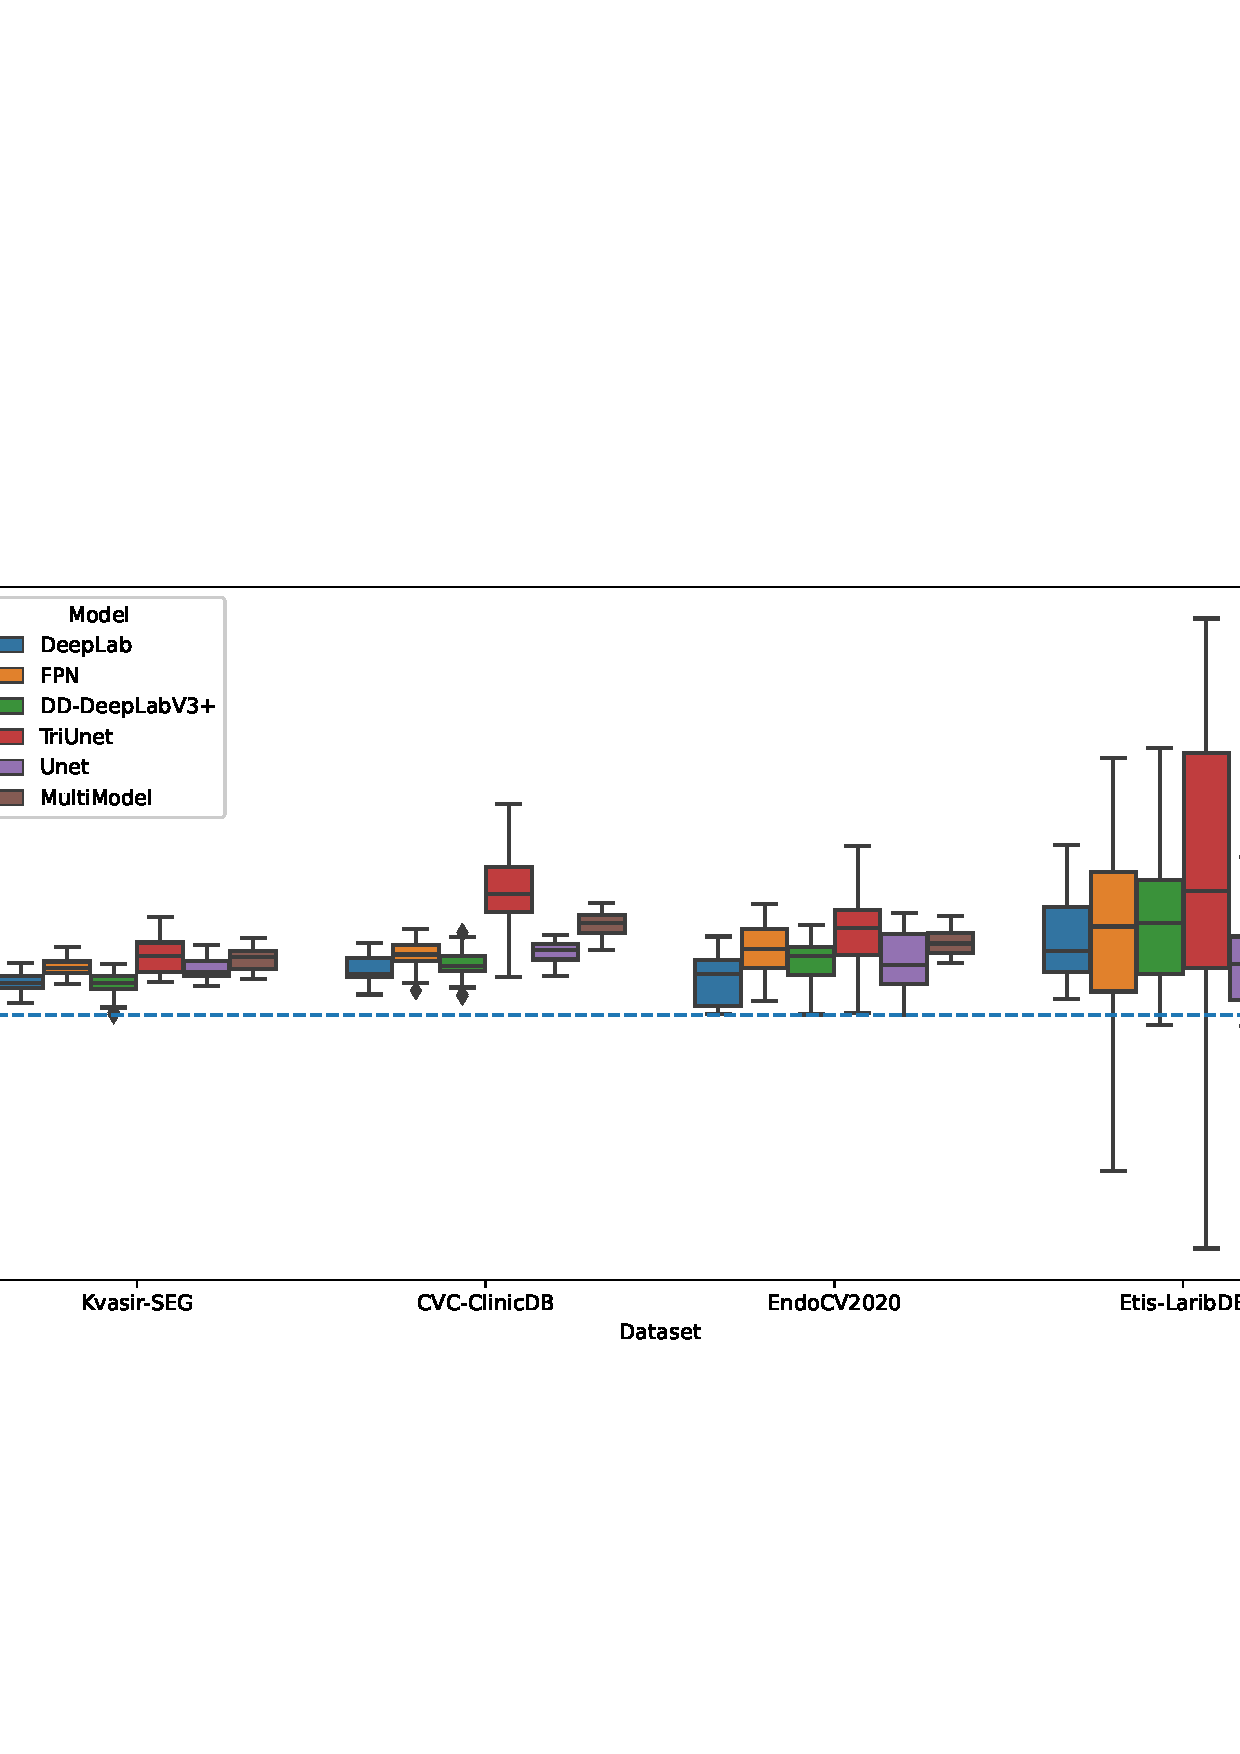
\includegraphics[width=\linewidth]{illustrations/improvements_due_to_ensembles.png}
    \caption[Improvements due to Ensembles]{Boxplot showing the improvement due to ensembles as a percentage of the mean \gls{iou} across their constituent models}
    \label{fig:ensemble_improvements}
\end{figure}
The \gls{iou}-scores for the ensemble models are shown in \Cref{tab:ensembles}. The relative improvements as a percentage of the constituent predictor performance is shown in \Cref{fig:ensemble_improvements}. The results show that ensembles increase generalization.  This, as mentioned in \Cref{background}, is often attributed to the fact that ensembles mitigate underspecification. Specifically, they constitute a form of Bayesian marginalization, and should thus in theory be able to leverage the variability of its constituent predictors in order to increase generalization.

To investigate the veracity of this line of reasoning, one can consider the relationship between the improvements to generalization due to the use of ensembles versus the performance variability of the constituent predictors. This is shown in \Cref{fig:ensemble_var} 
\begin{figure}[h]
    \centering
    \hspace*{-1.9cm}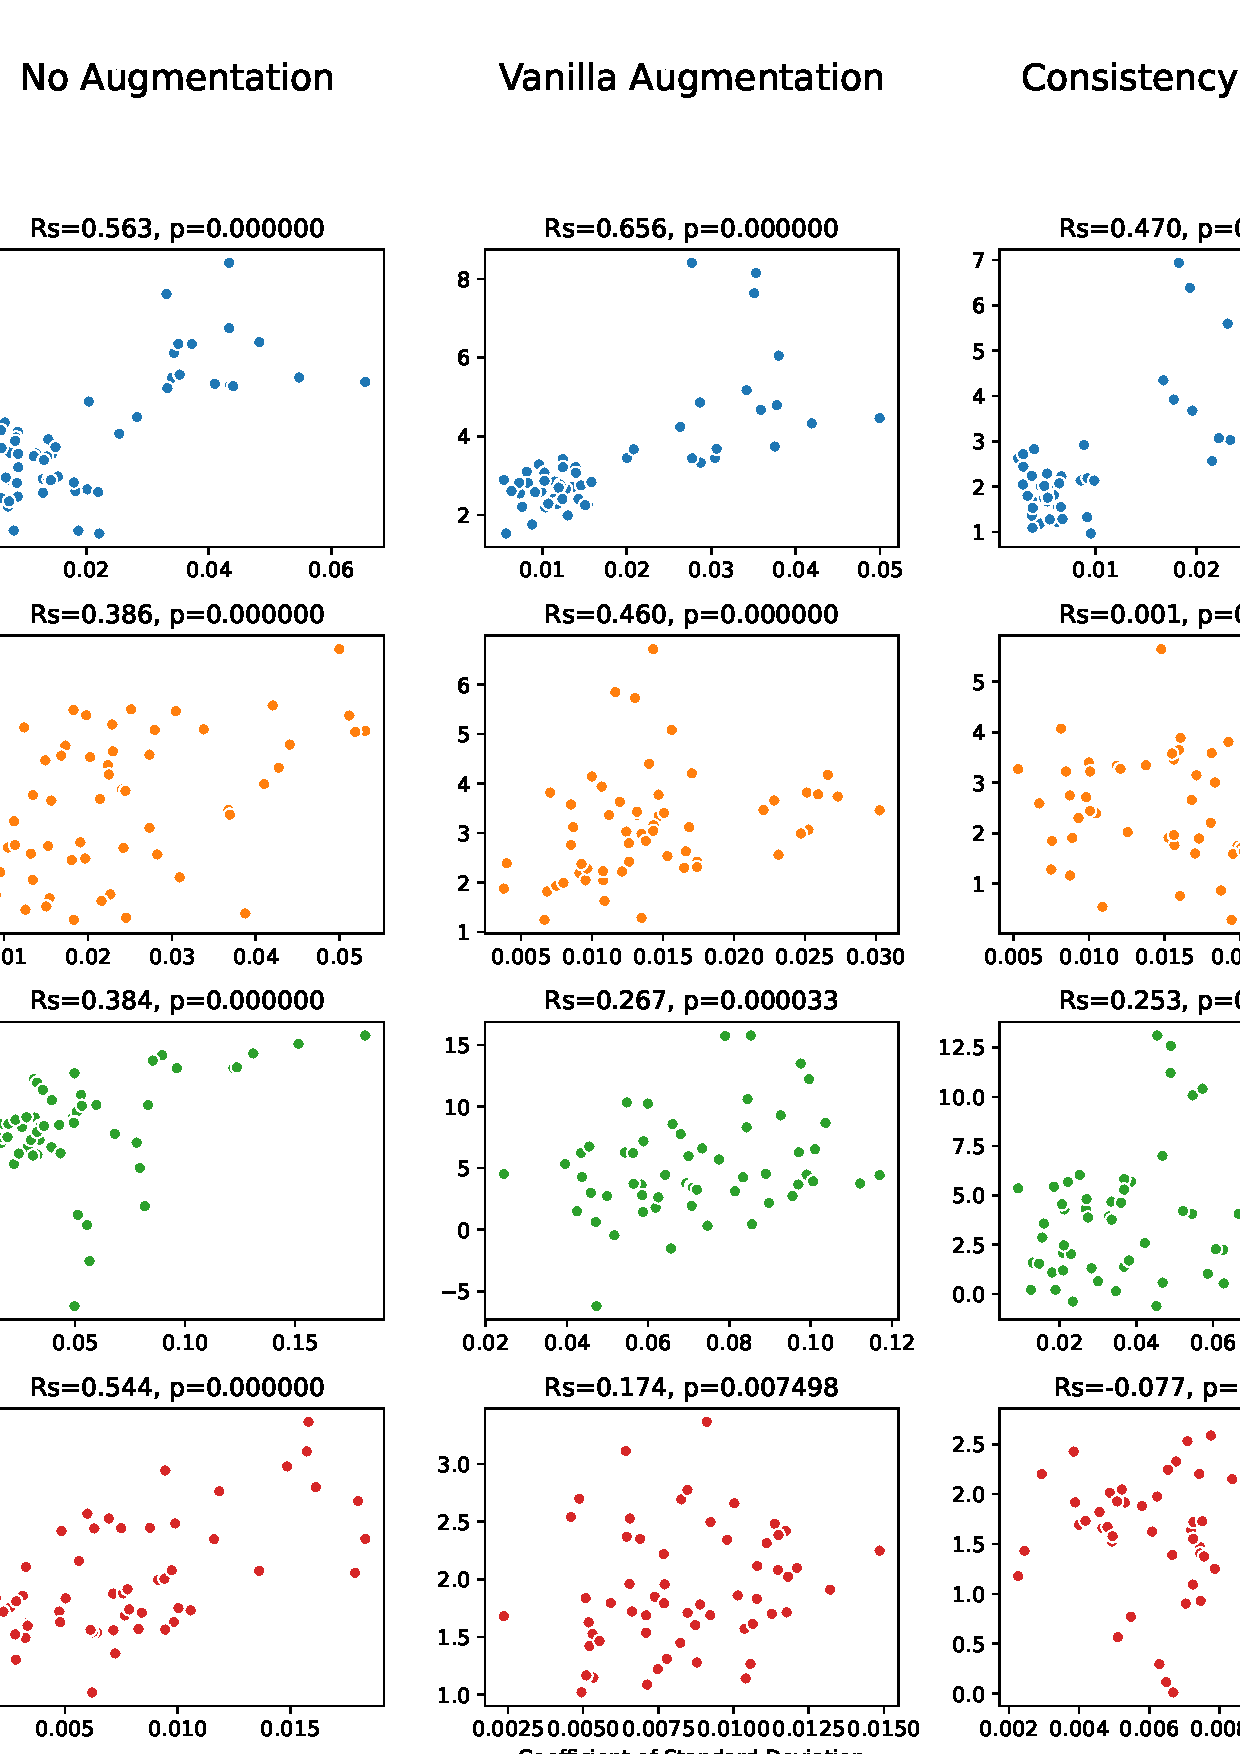
\includegraphics[width=1.2\linewidth]{illustrations/ensemble_variance_relationship_statistical.png}
    \caption[Relationship between ensemble improvements and constituents' performance variability]{Plot showing the correlation between the improvements to \gls{iou} with respect to the mean \gls{iou} of the constituent predictors, versus the variability in the performance of the constituent predictors. The Pearson Correlation Coefficient and corresponding p-value for each dataset is shown in the title of each subplot.}
    \label{fig:ensemble_var}
\end{figure}

The results do not appear to completely corroborate this analysis of why ensembles increase generalization, however. Though a Pearson correlation test reports positive correlations (p>0.99) on two of the datasets - CVC-ClinicDB and Etis-LaribDB - the relationship is nonetheless fairly spurious. This is likely to be due to the the nature of the landscape of the Bayesian posterior, as illustrated in \Cref{fig:bayesian_generalization} in \Cref{fig:bayesian_generalization}. Moreover, performance variability may not be an accurate representation of the degree to which the ensembles' constituent predictors encode different features. This will be discussed further in \Cref{discussion}. 


\section{Summary}
This chapter detailed the experiments performed to evaluate the methods presented in \Cref{methods} along with the effects of model architecture, augmentation, and ensembles on generalizability. The results can be summarized as follows:
\begin{itemize}
    \item Model architecture has limited bearing on increasing generalization, but large models are likely to harm it.
    \item Multitask learning as implemented using the Dual-decoder DeepLabV3+ had negligible impact, which may be attributed to the encoder learning dataset-agnostic features.
    \item Data augmentation increases generalization considerably, but the use of the generative inpainter had a negative effect.
    \item Consistency training outperforms conventional data augmentation, and increased generalization by significant margins on more difficult datasets.
    \item Ensembles models increase generalization, but not by as significant of a margin as one may expect based on the literature. The relationship between ensemble models and underspecification as quantified in this thesis is also somewhat more spurious than expected.
\end{itemize}
These findings will be discussed in further detail in \Cref{discussion}. 